\chapter{Herramientas Numericas} % Main chapter title

\label{SN} % For referencing the chapter elsewhere, use \ref{Chapter1} 

%----------------------------------------------------------------------------------------

% Define some commands to keep the formatting separated from the content 


Las simulaciones num\'ericas constituyen una de las herramientas mas importantes para el desarrollo de la astronom\'ia moderna. La enorme cantidad de particulas que constituyen por ejemplo una galaxia, hacen que los estudios an\'aliticos se vuelvan practicamente imposible. En este contexto es que cobra importancia un enfoque num\'erico de ciertos problemas constituidos por sistemas de muchas particulas y a\'un en estos casos se realizan aproximaciones. 
Aquellos sistemas que puedan ser descriptos como un fluido no collisional, permiten que los problemas se simplifiquen al poder lidiar con un conjunto muy reducido de particulas, conservando el comportamiento general del sistema. Dentro de este tipo de \textit{fluidos}, tenemos a las galaxias, sistemas de galaxias y a la materia oscura. CITA (Chandrasekhar 1943):? (Saas Springel? ). Por lo tanto, las simulaciones numericas cobran vital importancia en cosmolog\'ia por la practicidad que presentan. 


En este capitulo presentaremos una introducciones a la realizaci\'on de simulaciones numericas. Como generar sus condiciones iniciales y c..

\section{Simulaciones Num\'ericas}

\subsection{Din\'amica de macro particulas}

El modelo actual del universo es el de $\Lambda$CDM. Bajo este paradigma la materia del universo esta compuesta en casi $\sim 80 \% $ de materia oscura, y un $\sim 20 \% $ de materia bari\'onica. De modo que es esperable que la din\'amica general del universo este gobernada por lo que suceda con la materia oscura y que los bariones \textit{acompa\~nen} a la din\'amica de la materia oscura. 




Aca la idea es contar que en los fluidos no colisionales, como puede ser un universo descripto por materia oscura, un conjunto de macro particulas se comportan segun la ecuacion de Boltzman (desde donde se pueden recuperar las ecuaciones hidrodin\'amicas qeu voy a poner en la introduccion.)

Aca hacer una diferenciacion de cuando uno trabaja con particulas de gas o de materia oscura la integraci\'on va a ser diferente. 




\subsection{Condiciones Iniciales}
Tal como se vio en la secci\'on \ref{PerturbacionesLineales} la ecuaci\'on \ref{seriefourier}  nos permite representar a el contraste de densidad del universo como una superposici\'on de ondas de Fourier cuya amplitud viene dada por un espectro de potencias. Este espectro nos caracteriza el nivel de fluctuaciones a una dada escala espacial y puede medirse atrav\'es de relevamientos de galaxias. 

Generar condiciones iniciales para una simulaci\'on, consiste entonces en reproducir mediante una distribuci\'on de particulas el estado del universo temprano, para luego integrar las ecuaciones de movimiento de estas particulas, evolucionando asi el universo desde un estado temprano a alto redshift a el universo tal como lo conocemos hoy. 

De modo que en general, se utiliza la teor\'ia de perturbaciones lineales para generar el nivel de perturbaciones inicial, ya que a un redshift suficientemente alto, el universo a\'un estar\'ia en un r\'egimen lineal y ser\'ia v\'alida esta aproximaci\'on. Se generan entonces perturbaciones que tienen una amplitud conocida por el espectro de potencias pero una fase aleatoria. El hecho de qu eno podamos medir las fases de las perturbaciones del universo real hace que no podamos simular el universo real que habitamos. Por lo cual es importante resaltar que las simulaciones no constituyen una materializaci\'on del universo \textit{real}, sino que uno simula universos \textit{estad\'isticamente similares}. 

\subsection{Aproximaci\'on Zeldovich}

Podemos entonces escribir a las fluctuaciones de densidad en el espacio de Fourier donde entonces la fluctuacion en una escala k es:
\begin{equation}
    \hat{\delta}(k)=\delta_{k}e^{i\fi_{k}}
    \label{PerturbacionEscalaK}
\end{equation}{}
Donde la probabilidad de tener una fluctuaci\'on con una cierta fase y amplitud sigue una distribuci\'on exponencial en el cuadrado de $\delta_{k}$ y uniforme en la fase \textbf{Cita libro carlos}:
\begin{equation}
    P(\delta_{k},\phi_{k})=\frac{1}{2\sigma_{k}^{2}\pi}exp{(-\frac{\delta_{k}^{2}}{\sigma_{k}^{2}})^{2}}\delta_{k}d(\delta_{k}^{2})d\phi_{k}
  \label{ProbabilidadFluctuaciones}
\end{equation}{}
\begin{equation}
    \sigma_{k}^{2}=<\mid \hat{\delta}_{k}^{2} \mid >=P(k)
\end{equation}{}
Si uno escribe la perturbaci\'on \ref{PerturbacionEscalaK} como $\delta(k)=a_{k}+i b_{k}$ se puede demostrar que la ecuaci\'on \ref{ProbabilidadFluctuaciones} se transforma en una distribuci\'on Gausseana para $a_{k}$ y $b_{k}$ \textbf{cita libro carlos DODELSON}. Observaciones de el CMB \textbf{cITA?} permiten ver que las fluctuaciones de este son gauseanas, dando sustento a la teor\'ia. Al mismo tiempo, esta probabilidad de fluctuaciones esta predecida por las teor\'ias modernas de inflaci\'on. 

\begin{figure}
    \centering
    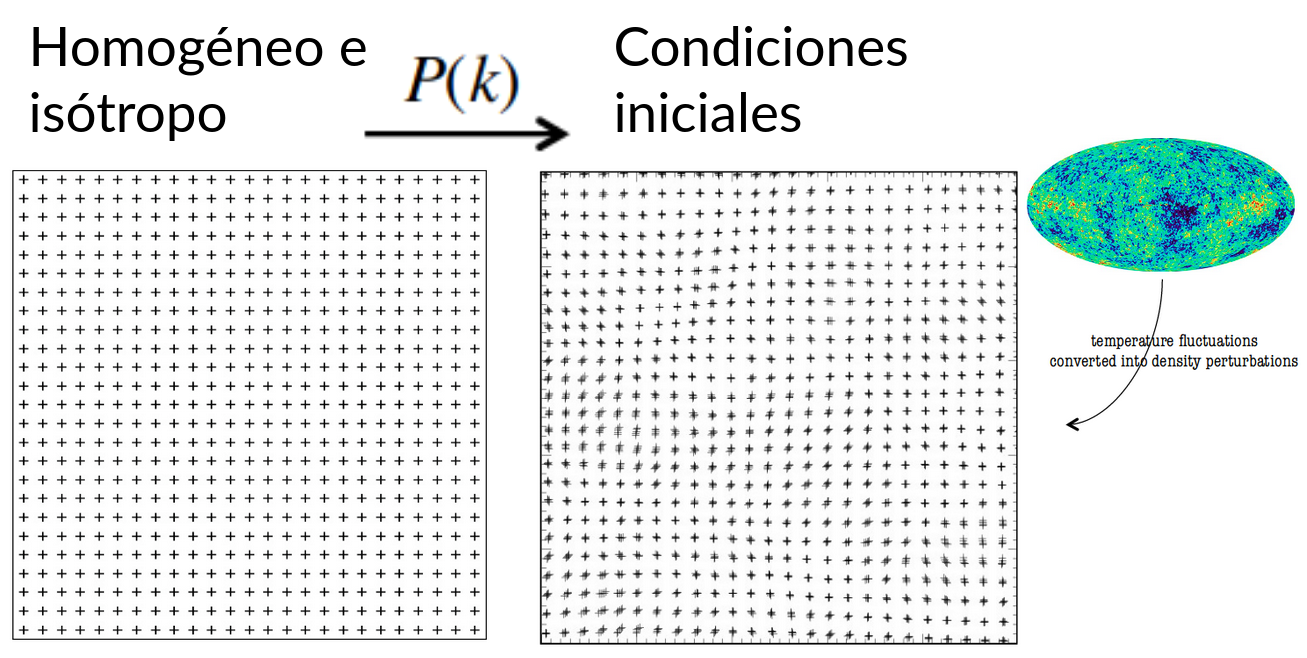
\includegraphics[width=12cm]{Figures/Captura de pantalla de 2020-01-11 16-26-38.png}
    \caption{\textbf{EDITA UNA IMAGEN CON ESTA ONDA. CITALO A KNEBE}}
    \label{Knebe}
\end{figure}{}

Lo que queremos hacer entonces es a partir de una distribuci\'on homogenea de particulas obtener una distribuci\'on que este levemente perturbada, cuyas fluctuaciones de densidad sean representativas de las de un universo temprano (figura \ref{Knebe}. Para esto se utiliza la \textit{Aproximaci\'on Zeldovich} \citep{Zeldovich1970}.

Esta consiste en obtener las posiciones $\textbf{x}(t)$ (denominadas posiciones eulerianas) a partir de las posiciones $\textbf{q}$ en una grilla homog\'enea (denominadas posiciones lagrangianas). La aproximaci\'on toma la forma dada por:

\begin{equation}
    \textbf{x}(t)=\textbf{q}+D(t)\textbf{S}(\textbf{q}) 
    \label{Zeldovich}
\end{equation}{}

La ecuaci\'on \ref{EcuacionDeltaAproximacion} se puede resolver num\'ericamente para obtener el valor de D(t). Esto es lo que comunmente se denomina \textit{Growth Factor} (Factor de crecimiento) que nos indica como se expande el universo con el tiempo y es una funci\'on que depende de la cosmolog\'ia que uno utilice.

El campo de desplazamiento \textbf{S}(\textbf{q} podemos escribirlo como el gradiente de un potencial \citep{Zeldovich1970}, y se puede demostrar que este potencial viene dado, a menos una constante, por las fluctuaciones de densidad $(\delta_{0})$. Entonces tenemos lo siguiente: 
\begin{equation}
    \textbf{S}(\textbf{q})=-\nabla\Psi
    \label{CampoS}
\end{equation}{}
\begin{equation}
    \nabla ^{2}\Psi=\delta_{0}
\end{equation}{}

En el espacio de Fourier esta ultima ecuaci\'on adopta una forma muy simple de:

\begin{equation}
    \hat{\Psi}=\frac{\hat{\delta}_{0}(k)}{k^{2}}
    \label{Transformadadelcampo}
\end{equation}{}

Tenemos entonces ahora todos los elementos para generar condiciones iniciales para una simulaci\'on. En resumen los pasos son los siguientes:
\begin{itemize}
    \item Dado un espectro de potencias P(k) voy a tener las amplitudes de las fluctuaciones a diferentes escalas espaciales.
    \item Vimos como son las probabilidades de obtener fluctuaciones de diferentes escalas, y si escribo $\delta(k)=a_{k} + i b_ {k}$ las probabilidades de $a_{k}$ y $b_{k}$ dependen de generar numeros aleatorios que sigan una distribuci\'on Normal.
    \item Habiendo generado las fluctuaciones puedo simplemente obtener el campo $\hat{Psi}$ siguiendo la ecuacion \ref{Transformadadelcampo}.
    \item Lo siguiente es antitransformar $\hat{\Psi}$ para obtener el campo en el espacio real $\Psi$.
    \item Y tomando el gradiente de este campo obtengo el campo de desplazamiento \textbf{S}. \ref{CampoS}
\end{itemize}{}

Las velocidades iniciales se obtienen facilmente derivando la ecuaci\'on \ref{Zeldovich}.
\begin{equation}
    \dot{\textbf{x}}=\dot{D}\textbf{S}(\textbf{q})
\end{equation}{}

\subsection{Limitaciones}
\label{Limitaciones}
Este m\'etodo tiene limitaciones que deben ser tenidas en cuenta a la hora de llevarlo a la practica. Estas son dos y vienen dadas por la cantidad de particulas que uno desee simular y por el tama\~no del \textit{box} cosmol\'ogico que uno utilice.

\begin{figure}
    \centering
    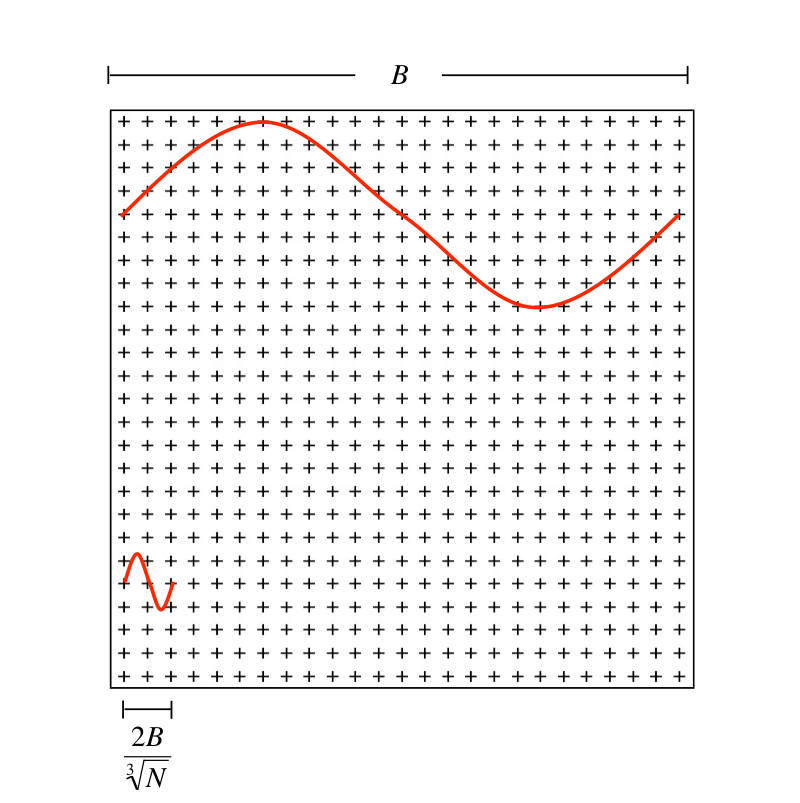
\includegraphics[width=12cm]{Figures/Captura de pantalla de 2019-10-02 17-37-57.png}
    \caption{Caption}
    \label{fig:my_label}
\end{figure}{}

Debido a que estamos reproduciendo una funci\'on en el espacio de fourier, las frecuencias mas largas que podemos reproducir vienen delimitadas por la regi\'on de periodicidad, que en nuestro caso es el tama\~no del \textit{box} que simulemos. 

Por otro lado, las frecuencias mas cortas que podamos reproducir estan delimitadas por el criterio de Niquist, y esto sera inversamente proporcional a la distancia media entreparticulas $^{3}\sqrt{N}$. Entonces cuantas mas particulas uno simule, la frecuencia de Niquist sera mas corta y asi podre simular frecuencias mas cortas. 


\subsection{Simulaci\'on}

Hasta aqu\'i hemos explicado como generar condiciones iniciales para una simulaci\'on. Estas condiciones iniciales comprenden a las posiciones y velocidades iniciales de las particulas. Lo siguiente entonces es integrar estas ecuaciones, para lo cual se utilizan c\'odigos de N-cuerpos. 

En el caso de que solo se simulen particulas de materia oscura, esta se movera solo por el campo gravitatorio generado por todas ellas. Este campo gravitatorio genera una potencial gravitatorio que genera a su vez una fuerza. Existen diversos m\'etodos para calcular los potenciales gravitarios, algunos de ellos son el \textit{particula-particula, Particle Mesh, TreePm, tecnicas de Fourier, etc.} 
Una elegante discusion de los diferentes m\'etodos es dada por \citet{SAAS}. 

\begin{figure}
 \centering
  \subfloat[Gatito]{
   \label{f:gato}
    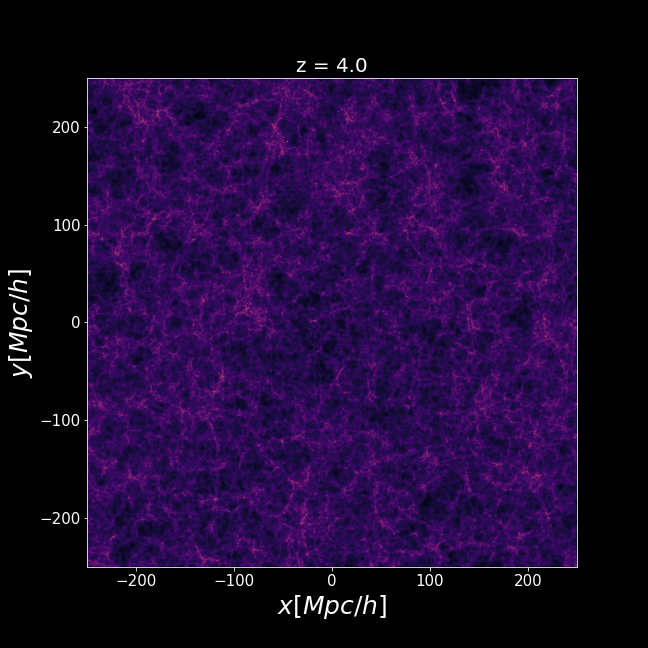
\includegraphics[width=0.3\textwidth]{Figures/base2.png}}
  \subfloat[Tigre]{
   \label{f:tigre}
    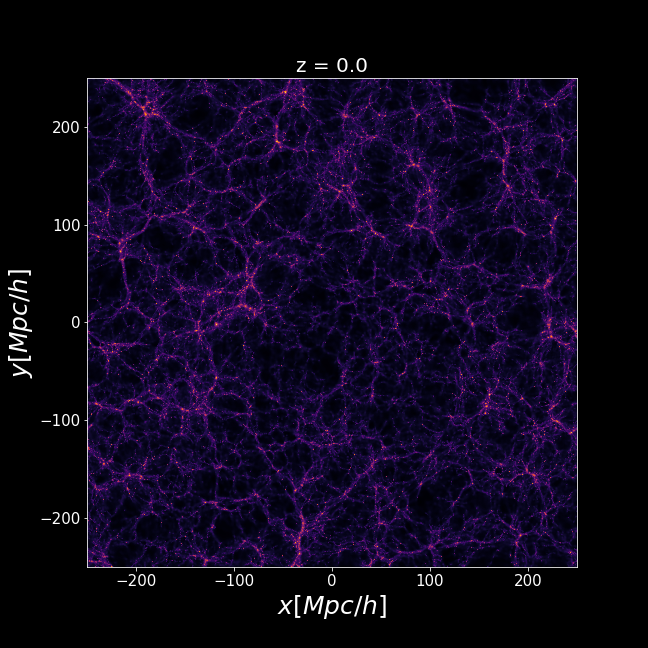
\includegraphics[width=0.3\textwidth]{Figures/base8.png}}
  
 \caption{Múltiples imágenes}
 \label{f:animales}
\end{figure}
 


\section{F\'isica Bari\'onica}

Los procesos astrof\'isicos que le ocurre a la materia barionica son de una enorme complejidad y dependen de una ampl\'isima gama de escalas. Por lo que implementarlos en un c\'odigo num\'erico requiere de un buen grado de model\'istica que var\'ia con las escalas que uno quiera estudiar. 

Principalmente en el universo los bariones se encuentran en estado gaseoso. A diferencia de la materia oscura, el gas se mueve no solo dominado por la gravedad sino que tambi\'en lo hace debido a los gradientes de presi\'on que generan fuerzas. Si queremos integrar entonces las ecuaciones de movimiento no solo de particulas de materia oscura, sino que tambi\'en particulas de gas, esto presenta una primera dificultad, ya que debemos ser capaces de generar a partir de particulas discretas campos \textit{continuos}, que puedan ser derivados para calcular propiedades (como la presi\'on). Existen diversas maneras de hacer esto, una de las mas importantes es lo que se conoce como \textbf{Smooth particle hidrodynamics} (\textit{SPH}) o en espa\~nol, \textit{Hidrodin\'amica de particulas suavizadas}.

\subsection{Hidrodin\'amica de particulas suavizadas}
\label{SPH}

\citet{Gingold1977} desarrollaron una manera de representar propiedades continuas de fluidos atrav\'es del uso de particulas. Esta t\'ecnica que originalmente se penso para el uso de c\'odigo magnetohidrodin\'amicos, pronto se popularizaron para el uso de calculos astrof\'isicos. La idea es simple y consiste en interpolar las propiedades en el espacio mediante el uso de un \textit{Kernel}. Se representa entonces cualquier campo \textbf{F}(\textbf{r} de la siguiente manera:
\begin{equation}
    \textbf{F}(\textbf{r})=\int \textbf{F}(\textbf{r}')W(\textbf{r}-\textbf{r}',h)d\textbf{r}'
    \label{IntegralSPH}
\end{equation}{}

La funci\'on W es el \textit{Kernel Interpolatorio}, normalmente se utilizan funciones de soporte compacto, como un spline c\'ubico. La variable h es el \textit{ancho} del kernel. Para ser factible implementar este m\'etodo en un c\'odigo num\'erico debemos discretizar la integral \ref{IntegralSPH}. Para particulas con una masa $m_{i}$ y una densidad $\rho_{j}$ podemos asignarles un \textit{volumen caracteristico} $V_{i}\sim m_{j}/\rho_{j}$ que utilizaremos como diferencial de volumen, entonces la ecuacion \ref{IntegralSPH} se aproxima de la siguiente manera:
\begin{equation}
    \textbf{F}(\textbf{r})\simeq \sum_{j} \frac{m_{j}}{\rho_{j}} F_{j} W(\textbf{r}-\textbf{r}_{j},h)
    \label{IntegralSPHDiscreta}
\end{equation}{}

\ref{IntegralSPHDiscreta} es una integral en el sentido \textit{Monte Carlo}. Para tener una buena estima de el valor del campo \textbf{F} en el punto \textbf{r} un debe efectuar la suma sobre una cantidad adecuada de particulas. Por supuesto que la mejor estima se obtiene al realizar la suma sobre todas las particulas, pero esto es num\'ericamente costoso. Realizar la suma sobre una cantidad $n\sim30$ genera una buena estima del campo. C\'odigos mas modernos como \texttt{\textbf{GIZMO}} la realizan sobre las 56 vecinas mas cercanas \citep{GIZMO2015}.

Por ultimo, para realizar la interpolaci\'on la variable h de el \textit{Kernel} W normalmente es la distancia a la n-\'esima vecina mas cercana. El \textit{Kernel} es tal que si $h\rightarrow 0$ $W \rightarrow \delta_{dirac}$, esto produce que una determinada propiedaded este localizada en un entorno peque\~no, mientras que si h es \textit{grande} las propiedades se distribuyen ampliamente en el espacio. 

\subsection{Modelos Astrof\'isicos \textit{Subgrid}}

La t\'ecnica de SPH, asi como otros m\'etodos como el particle mesh, adaptative mesh \textbf{CITAS} permiten integrar las ecuaciones de particulas de gas y de esta manera seguir su din\'amica. Ahora bien, procesos sumamente complejos producen que los bariones colapsen y formen nebulosas, a su vez estas formen estrellas que luego explotan como supernovas, estas aumentan la temperatura del gas circundante, se forman agujeros negros, y muchisimos otros procesos que ocurren a escalas mucho mas all\'a de las que pueden resolver las computadoras mas modernas. Debido entonces a que interacciones de estas escalas no pueden resolverse directamente en simulaciones cosmologicas se implementan otras alternativas para poder estudiar las propiedades bari\'onicas del universo.

Para poder reproducir fen\'omenos astrof\'isicos en simulaciones cosmologicas se implementan lo que se conoce como modelos \textit{sub-grid}. La idea es reproducir fen\'omenos que ocurren mas all\'a de el nivel de resoluci\'on de la simulaci\'on. Estos modelos reproducen en un sentido estad\'istico las propiedades barionicas del universo. 

La cantidad de modelos es muy ampl\'ia y abarca una amplia gama de complejidad. Aqu\'i se explican los principios b\'asicos sobre los que se calculan propiedades bari\'onicas en el modelo de \citet{Springel2003}.
La idea es que las particulas de SPH tienen una \textit{parte} de poblaci\'on condensada (c) que se encuentra en presi\'on de equilibrio y otra \textit{parte} caliente (h). Las nubes frias o poblaci\'on condensada proveen el material disponble para la formaci\'on estelar. En estas particulas \textit{hibridas} solo la poblaci\'on caliente esta sujeta a las ecuaciones d ela hidrodin\'amica. La parte fria interactua bajo gravedad pero si participa en los intercambios de energ\'ia y masa con la fase caliente. De modo que la densidad total de una particula de gas es la suma de las densidades de las dos poblaciones. 
\begin{equation}
    \rho = \rho_{h} + \rho_{c}
\end{equation}{}
Se modelan entonces 3 procesos que intercabian masa y energ\'ia entre las 2 fases.
\begin{itemize}
    \item \textbf{Formaci\'on Estelar}: 
    \begin{equation}
        \frac{d{\rho_{\star}}}{d{t}}=\frac{\rho_{c}}{t_{\star}}-\beta\frac{\rho_{c}}{t_{\star}}
    \end{equation}{}
    $t_{\star}$ representa un tiempo caracteristico en que las nubes fr\'ias convierten estrellas y $\beta$ es la fracci\'on de las estrellas m\'asivas que se forman. Estas estrellas tienen tiempos de vida muy cortos e instant\'aneamente explotan como supernovas. Tanto $\beta$ como $t_{\star}$ son par\'ametros del modelo. Notese que la fracci\'on $\beta$ que produce supernovas va a generar instant\'aneamente un intercambio de energ\'ia mediante \textit{feedback}. 
    
    \item \textbf{Calentamiento por \textit{feedback}}
    \begin{equation}
    \frac{d}{dt}(\rho_{h}u_{h})|_{SN}=\epsilon_{SN}\frac{d\rho_{\star}}{dt}=\beta u_{SN}\frac{\rho_{c}}{t_{\star}}
    \end{equation}{}
    
    $\epsilon_{SN}$ es la cantidad de energ\'ia que libera una supernova y es otro par\'ametro del modelo. El calentamiento producido por las supernovas lo que va a producir es un aumento de la energ\'ia interna (u) de las particulas cercanas, calentando de esta manera la fase caliente de las particulas.
    
    Este aumento de temperatura va a producir que las nubes fr\'ias se evaporen, retornando de esta manera material a la fase caliente. 
    \begin{equation}
        \frac{d\rho_{c}}{dt_{\star}}=A\beta\frac{\rho_{c}}{t_{\star}}
    \end{equation}{}
    donde A es la eficiencia de evaporaci\'on y tambi\'en constituye un par\'ametro del modelo. 
    
    \item \textbf{Crecimiento de nubes frias}: 
    \begin{equation}
        \frac{d\rho_{c}}{dt}|_{TI}=-\frac{d\rho_{h}}{dt}|_{TI}=\frac{1}{u_{h}-u_{c}}\Lambda_{net}(\rho_{h},u_{h})
    \end{equation}{}
    La fase caliente va a producir procesos radiativos que van a producir un enfriamiento (\textit{cooling}) generando de esta manera que el gas caliente se transforme en gas frio. Este proceso va a depender de la \textit{Funci\'on de cooling} $\Lambda_{net}$ que uno implemente. 
    
\end{itemize}{}

As\'i de esta manera el modelo lo que produce es un intercambio entre las fases de gas que es autoregulatorio y reproduce estad\'isticamente propiedades astrof\'isicas del universo. En un esquema general, cuando la poblaci\'on de gas fr\'io sea lo suficientemente grande se formaran estrellas. Estas produciran supernovas que reinsertaran energ\'ia al ambiente por \textit{feedback} calentando de esta manera el gas. Este gas caliente comenzara a radiar y de esta manera se enfriara, aumentan la poblaci\'on caliente, y el ciclo se reanuda. 

El esquema aqui presentado es el correspondiente a \citet{Springel2003} y constituye uno de los mas simples modelos subgrid. Existen muchisimos modelos que reproducen otros fen\'omenos que aqu\'i se ignoran como por ejemplo la formaci\'on de agujeros negros supermasivos \textcolor{red}{textbf{BUSCAR CITA}} introduciendo otros tipos de feedback mas complejos. 

\section{Re-simulaciones }

En la secci\'on \ref{Limitaciones} se indico cuales eran las limitaciones que existen a la hora de realizar simulaciones y estas eran el tama\~no del \textit{box} y la cantidad de particulas que se utilicen. Si uno obtiene en un \textit{box peque\~no} una cantidad \textit{grande} de particulas, uno va a tener una simulaci\'on de mucha resoluci\'on. La resoluci\'on se refiere a la masa de las particulas que uno tenga, si esta masa disminuye entonces uno gana resoluci\'on, ya que va a poder muestrear una misma estructura con mas particulas, ganando asi detalles. 

Entonces si uno quiere hacer una simulaci\'on con mucha resoluci\'on va a tener que poner la mayor cantidad de particulas que pueda en su \textit{box}. Esto va a generar un problema ya que cuanto mas particulas uno quiera simular, mayor sera el tiempo de computo que uno requiera para integrar sus ecuaciones de movimientos. Existen situaciones en cambio en que a uno puede interesarle tener mucha resoluci\'on en tan solo una regi\'on de el \textit{box} y poca en otra. En estos casos se utiliza la t\'ecnica de \textit{Re-simulaciones} o simulaciones \textit{Zoom-in}. Por ejemplo uno querr\'ia simular un cumulo, y tener mucha resoluci\'on en la galaxia central y el resto de las galaxias miembros del grupo tenerlas solo para que ejerzan efectos tidales sobre la central. 

En general, la resimulaci\'on consiste en identificar en una simulaci\'on una regi\'on que a uno le interese, y luego volver a realizar la simulaci\'on pero obteniendo mas resoluci\'on en esa regi\'on. Entonces realizar una re-simulacion consta de al menos dos etapas. Primero se genera una simulaci\'on \textit{base} y luego se realiza al re-simulaci\'on en todo el \textit{box} original, con mayor resoluci\'on en alguna regi\'on. 

Para poder realizar esto, uno tiene que a las condiciones iniciales de la simulaci\'on \textit{base} agregarle perturbaciones de escalas mas chicas. En la regi\'on de inter\'es se agregan al mismo tiempo mas particulas disminuyendo asi la distancia media entre particulas. De esta manera en esta regi\'on las particulas seran sensibles a las nuevas perturbaciones que se agregaron en las condidiones iniciales.

Luego se vuelven a integrar las ecuaciones de movimientos de todas las particulas y el resultado final es la obtenci\'on de mayor resoluci\'on en la regi\'on de inter\'es. 




\begin{figure}
 \centering
  \subfloat[Gatito]{
   \label{f:gato}
    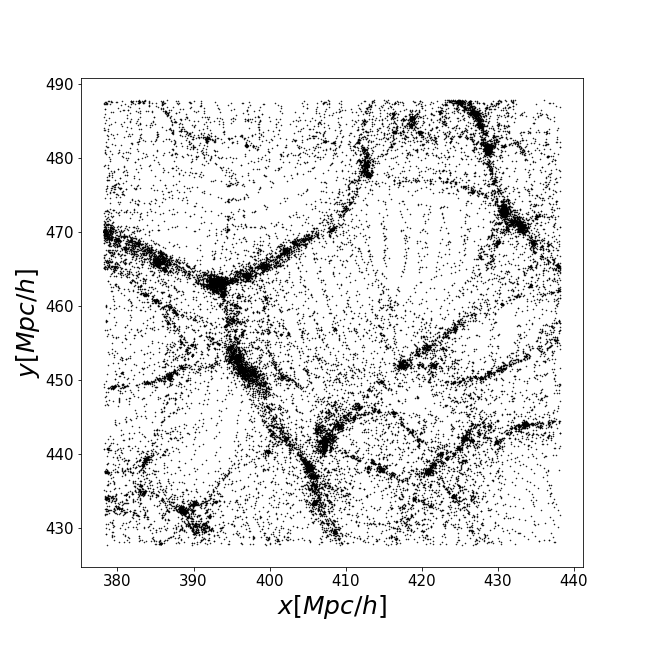
\includegraphics[width=0.3\textwidth]{Figures/proceso1.png}}
  \subfloat[Tigre]{
   \label{f:tigre}
    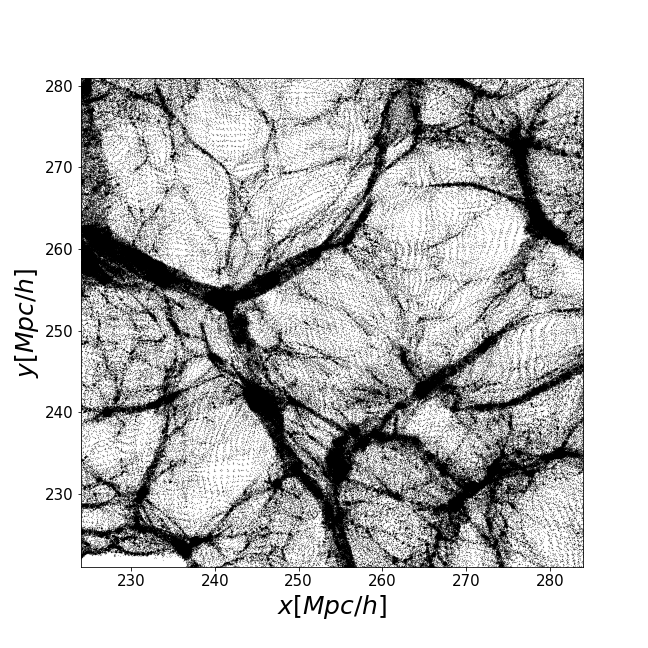
\includegraphics[width=0.3\textwidth]{Figures/proceso6.png}}
  
 \caption{Múltiples imágenes}
 \label{Resimulacion}
 
\end{figure}
 

La figura \ref{Resimulacion} presenta una simulaci\'on zoom-in realizada sobre un \textit{box} de 500 Mpc de lado. La imagen de el lado derecho es la resimulacion de la regi\'on de inter\'es (izquierda). Se puede observar que la resoluci\'on alcanzada es de mayor grado permitiendo de esta manera obtener mayor nivel de detalle. Pero en terminos generales las estructuras son las mismas, solo que con resouciones diferentes. 



\section{Halos de materia oscura}

Las particulas de materia oscura forman estructuras virializadas que se conocen como \textbf{halos}. Es en estas regiones donde los bariones colapsan para formar las galaxias. Por lo cual las estructuras trazadas por halos de materia oscura en las simulaciones deben ser an\'alogas a aquellas trazadas por galaxias. Existen diversos c\'odigos num\'ericos que identifican los halos en simulaciones y estos se construyen sobre diferentes fundamentos te\'oricos. A lo largo de este trabajo utilizaremos el c\'odigo \texttt{ROCKSTAR} desarrollado por \citet{Rockstar}  para la identificaci\'o de los halos de materia oscura en las simulaciones. Es importante destacar que este c\'odigo solo trabaja sobre las particulas de materia oscura. 


\section{Identificaci\'on}

Para identificar vac\'ios existen diferentes criterios, nosotros utilizamos el m\'etodo de \citep{Ruiz2015} donde los voids se definen como estructuras esf\'ericas cuyo contras de densidad integrado, definido por:
\begin{equation}
    \Delta(r)=\frac{3}{r^{3}}\int_ {0}^{r}\delta(r')r'^{2}dr'
    \label{ContrasteDensidadIntegrada}
\end{equation}{}
es de $\Delta=-0.9$.

El algoritmo trabaja de la siguiente manera:
\begin{itemize}
    \item Se comienza realizando una teselaci\'on de Voronoi sobre el cat\'alogo de halos o galaxias. Esta teselaci\'on consiste en calcular para cada punto trazador (halos) la regi\'on que esta mas cerca de este que de otro trazador.
    \item Se estima el campo de densidad, que consistira en $\rho_{celda}=\frac{1}{area celda}$. 
    \item Luego se eligira como candidatos a voids aquellas celdas que contengan una $\delta_ {celda}<-0.8$
    \item Se calcula el contraste de densidad integrada \ref{ContrasteDensidadIntegrada} en esferas alrededor de los trazadores seleccionados, hasta que alcancen $\Delta=-0.9$
    \item Mediante una caminata aleatoria alrededor de los trazadores se relocaliza un nuevo centro, desde donde se comienza a integrar el contraste $\Delta$ nuevamente. Si este alcanza $\Delta=-0.9$ a un radio mayor, se lo fija como nuevo centro.
    
\end{itemize}{}
De esta manera se hace iterativamente hasta lograr convergencia. 